\subsubsubsubsection{Bikepath}
\begin{figure}[h]
\centering
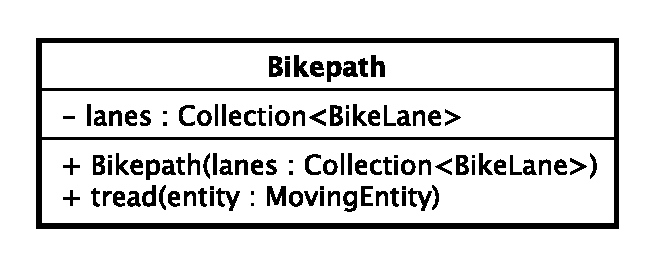
\includegraphics[scale=0.6,keepaspectratio]{images/solution/bikepath.eps}
\caption{App::Reactive::Bikepath}
\label{fig:sd-app-bikepath}
\end{figure}
\FloatBarrier
\begin{itemize}
  \item \textbf{Description} \\
    It represents a concrete bikepath which is composed by at least one lane.
  \item \textbf{Attribute}
  \begin{itemize}
    \item \texttt{- lane: ArrayList<BikeLane>} \\
A bikepath is composed by lanes.
  \end{itemize}
  \item \textbf{Operation}
  \begin{itemize} 
    \item \texttt{+ tread(entity: MovingEntity)} \\
Moves the entity on the correct lane based on the current entity route. 
  \end{itemize}
\end{itemize}
